\documentclass[11pt]{article}

\usepackage[T1]{fontenc}
\usepackage[utf8]{inputenc}
\usepackage{mathptmx}
\usepackage{courier}
\usepackage[margin=1in]{geometry}
\usepackage{microtype}
\usepackage{amsmath,amssymb}
\usepackage{booktabs}
\usepackage{tabularx}
\usepackage{graphicx}
\usepackage{xcolor}
\usepackage{caption}
\usepackage{enumitem}
\usepackage{tikz}
\usetikzlibrary{arrows.meta,positioning,calc}
\usepackage[numbers,sort&compress]{natbib}
\usepackage[hidelinks]{hyperref}
\usepackage{url}

\captionsetup{font=small,labelfont=bf}
\setlist{itemsep=2pt,topsep=4pt}
\newcommand{\tabsize}{\footnotesize}

\title{Into the Trenches: Predicting Memecoin Pumps\\Seconds Before They Start}
\author{Ronith Sharmila\\
Southwestern Oklahoma State University\\
ronith.sharmila@swosu.edu}
\date{}

\begin{document}
\maketitle

\begin{abstract}
Hundreds of thousands of new tokens are created every month on memecoin launchpads such as pump.fun, where creating a tradable token takes only seconds. While most of these tokens die quickly, some undergo a surge: a sudden, short-lived and substantial increase in price. We study whether the onset of a surge can be predicted seconds in advance using only on-chain information that is available at the time of prediction. We construct a point-in-time benchmark with 8.4 million observations of 622,303 pump.fun tokens created between 5 June and 14 July 2026. Surge onset is defined with a prespecified detector, and the final week of data remained unseen until a single, preregistered scoring run. On this held-out week, a gradient-boosted tree model ranks observations with an ROC-AUC of 0.866 in predicting whether a surge will start within the next 60 seconds. Observations in its top 1\% contain surge onsets 6.3 times more often than the base rate, with a median lead time of about five seconds. Prediction is harder among actively trading tokens, where the ROC-AUC is 0.768; this is substantially lower than 0.866 but still well above chance. The choice of model matters little: an L2-regularized logistic regression on the same 124 causal features performs similarly, while a 10-million-parameter multimodal Transformer with self-supervised pretraining performs worse. We also caution that predictability does not imply profitability: during the validation week, tokens with scores in the top 1\% had a median return of $-40\%$ over the next five minutes. Finally, we document how future information leaking through a cost-saving sampling of transactions inflated ROC-AUC from 0.835 to 0.917 on a subset of the data, and we describe the checks that exposed it.
\end{abstract}

\section{Introduction}
\label{sec:intro}

A launchpad is a platform that lets users create their own cryptocurrencies. On pump.fun, the largest launchpad on Solana, any user can create a token by choosing a name, a ticker and an image, with no need to write or deploy a smart contract. Tokens created on pump.fun trade on a bonding curve, which sets the price from the first trade onward. As a result, these launchpads produce an enormous number of small, new cryptocurrencies. One study of pump.fun counts about 15 million coins launched over two years~\citep{szwajcok2026factories}, while another finds that fewer than 2\% of the platform's tokens reach a major decentralized exchange~\citep{mancino2025memecoin}. In the public corpus we use, about 0.7\% of launched tokens graduated from the bonding curve during our 39-day window~\citep{slinkdev2026corpus}.

For most of these tokens, trading dries up after a handful of transactions and they are forgotten. For a small subset, however, the price surges: within a few seconds, strong buying pressure drives a steep, abrupt rise, which typically fades within minutes. In a stratified sample of tokens from our data, the median surge peaked 73\% above its starting price about 32 seconds after it began. Such surges attract retail traders and automated trading bots, and some are the product of coordinated manipulation~\citep{szwajcok2026factories,mongardini2025midsummer}. Understanding and predicting them therefore matters to traders, to platforms and wallet applications deciding whether to warn users, and to researchers and regulators.

Prior work has studied this market from several angles. Measurement studies describe the platform, its graduation dynamics and the manipulation strategies used on it~\citep{mancino2025memecoin,kamat2026auditing,szwajcok2026factories}. Predictive studies estimate whether a token will graduate from its bonding curve~\citep{marino2026predicting}, flag likely rug pulls from the first minutes of trading~\citep{li2026catching}, or identify high-risk launches before they migrate to an exchange~\citep{hu2026melt}. A separate line of work studies pump-and-dump schemes on centralized exchanges, which are typically organized in advance on platforms such as Telegram~\citep{kamps2018moon,xu2019anatomy,hu2023sequence}. Detection systems spot such pumps seconds after they start~\citep{lamorgia2020pump,lamorgia2023doge}, and recent work ranks likely target coins shortly before an announced pump~\citep{bolz2024realtime}. Our work differs from all of these in one important way: we ask whether a surge is about to begin, within seconds, at any arbitrary point in a token's life, using only on-chain data. To our knowledge, this prediction task has not been studied before. \citet{marino2026predicting}, for instance, predict graduation and explicitly leave prediction of the pump itself to future work.

This question is easy to get wrong. Labels depend on the future by construction, features computed from on-chain data can quietly include future information, and the market changes from week to week. We therefore put as much effort into the evaluation protocol as into the models. All model and hyperparameter choices were made on walk-forward folds inside the training period. A separate validation week was used for development reporting. The final week was locked until we had written down, and committed to version control, exactly which models and metrics we would report. We then scored it once.

Our contributions are as follows.
\begin{enumerate}
  \item \textbf{A task and benchmark.} We formulate seconds-ahead surge-onset prediction on a bonding-curve launchpad, and we build a point-in-time dataset of 8.4 million observations of 622,303 pump.fun tokens with a prespecified surge detector, causal observation sampling and chronological, token-disjoint splits.
  \item \textbf{A preregistered evaluation.} We evaluate five model families on a locked final week, scored once under a protocol committed before the test data were read. We report token-clustered confidence intervals, lead times, event-level recall and results within strata of token age and activity.
  \item \textbf{A predictability result.} Surge onset is predictable from causal on-chain state. On the held-out week, the best model reaches an ROC-AUC of 0.866 at a 60-second horizon and 0.768 among actively traded tokens, and its top-ranked observations contain surge onsets at about six times the base rate.
  \item \textbf{A model-family comparison.} Gradient-boosted trees and L2-regularized logistic regression perform almost identically on the same engineered features, and neither wins in every subgroup. A multimodal Transformer trained on raw event sequences, with self-supervised pretraining, performs worse than both overall.
  \item \textbf{A leakage case study.} We show how a reasonable-looking, cost-driven choice of which transactions to fetch from an RPC node leaked future information and inflated a model's ROC-AUC from 0.835 to 0.917, even though every individual record passed timestamp checks. We also describe a separate evaluation bug and the tests that caught both problems.
\end{enumerate}

We also find that predictability and profitability are different things. The observations our model ranks highest are, on average, followed by steep losses, which is consistent with a market where any easily detected edge is short-lived. We do not offer a trading strategy, and we discuss the dual-use risks of this kind of model in Section~\ref{sec:discussion}.

Section~\ref{sec:background} explains how pump.fun works and Section~\ref{sec:related} reviews related work. Sections~\ref{sec:problem}--\ref{sec:protocol} define the task, the data, the models and the evaluation protocol. Section~\ref{sec:results} reports results, Section~\ref{sec:leakage} presents the leakage case study, Section~\ref{sec:discussion} discusses implications, limitations and ethics, and Section~\ref{sec:conclusion} concludes.

\section{Background: How a pump.fun Token Trades}
\label{sec:background}

When a token is launched on pump.fun, its supply is fixed and placed in a bonding curve, a smart contract that initially serves as the token's only market maker. The curve maintains virtual reserves of both the token and SOL, and the ratio between these reserves sets the marginal price. Buying a token adds SOL to the curve and removes tokens, pushing the price higher along a predetermined path; selling does the opposite. A token's price on the curve can therefore be deduced from the amount of SOL that has gone into it, and ``curve progress'', the share of the sellable supply already bought, is a natural summary of where a token stands.

When enough SOL has accumulated, the curve completes and the token \emph{graduates}: its liquidity migrates to a conventional automated market maker. Since March 2025 the destination has been PumpSwap, the platform's own exchange; before that it was Raydium~\citep{theblock2025pumpswap}. Graduation is rare, and most tokens never get there.

Every trade on the curve is a Solana transaction, so the full trading history of every token is public. Trade records include the trader's wallet, the direction and size of the trade, and the state of the curve after the trade. Two properties of this market shape our task. First, it is fast: tokens live and die within minutes, and much of the trading is done by bots. Second, the information is public but fragmented. The trade tape of a single token is easy to obtain, but richer context, such as transaction-level fee data, token-balance changes and wallet histories, has to be assembled from additional sources, often at a cost. Section~\ref{sec:leakage} shows why that cost matters.

\section{Related Work}
\label{sec:related}

\paragraph{Memecoin and launchpad measurement.}
\citet{mancino2025memecoin} describes pump.fun's growth in late 2024 and its share of Solana token creation and trading. \citet{kamat2026auditing} studies graduation on pump.fun with survival models and audits how reliable collector-generated graduation labels are. \citet{szwajcok2026factories} document five manipulation strategies on pump.fun, including wash trading and coordinated selling, as well as a market for manipulation-as-a-service tools. \citet{mongardini2025midsummer} study memecoins across several chains and find signs of artificial activity in most high-return tokens. \citet{cernera2023token} study token launches, rug pulls and sniper bots on Ethereum and BNB Smart Chain. These studies describe the market we model but do not forecast price surges.

\paragraph{Early prediction on launchpads.}
\citet{marino2026predicting} estimate the probability that a pump.fun token graduates, conditional on how much SOL its curve holds and on behavioral covariates, and leave prediction of the pump leg to future work. \citet{li2026catching} predict rug pulls on Solana from the first five minutes of trading and find that XGBoost works best. \citet{hu2026melt} build a behavioral dataset of launchpad tokens and predict which will become high-risk after migration. CoinCLIP~\citep{long2024coinclip} combines on-chain data with images and text to judge memecoin viability. Our task differs in its target, a price surge rather than graduation, fraud or long-run viability, and in its timing: we predict at many points in a token's life, seconds ahead.

\paragraph{Pump-and-dump detection.}
On centralized exchanges, pump-and-dump schemes are typically organized in advance in Telegram groups. \citet{kamps2018moon} propose detection criteria. \citet{xu2019anatomy} predict which coin a group will pump. \citet{lamorgia2020pump,lamorgia2023doge} detect pumps in real time, seconds after they start. \citet{hu2023sequence} predict target coins from sequences of past pumps. \citet{bolz2024realtime} rank candidate coins shortly before an announced pump. These settings have an organizer, an announcement time and a short list of candidate coins. Launchpad surges have none of these, and the candidate set is every live token.

\paragraph{Trees versus deep learning on tabular data.}
Several benchmarks find that gradient-boosted trees match or beat deep models on tabular data~\citep{grinsztajn2022tree,shwartzziv2022tabular,mcelfresh2023neural}. Our model-family result is consistent with that literature in a setting where the deep model also had access to raw event sequences.

\paragraph{Leakage and evaluation practice.}
\citet{kapoor2023leakage} survey how data leakage has inflated results across machine-learning-based science. In finance, \citet{lopezdeprado2018advances} discusses leakage across time and proposes purged cross-validation. Preregistration is standard in parts of the empirical sciences~\citep{nosek2018preregistration} but rare in machine learning for crypto markets. Our case study adds a specific, hard-to-spot mechanism, selection leakage in the acquisition of on-chain data, together with practical tests for it.

\section{Problem Formulation}
\label{sec:problem}

\paragraph{Observations.}
Let token $i$ be launched at time $L_i$. An observation is a pair $(i, T)$ with $T \ge L_i$. The information available at $T$ consists of all on-chain events for token $i$ with timestamps up to $T$, together with market-wide context from completed time intervals before $T$. A model maps this information to a score, and every feature must be computable at $T$ without any later data.

\paragraph{Surge onset.}
We detect surges from each token's trade stream with a rule-based detector whose parameters were fixed before any model was trained. Under the primary definition, a trade at time $t_0$ marks a surge onset if all of the following hold:
\begin{itemize}
  \item the 30 seconds starting at $t_0$ contain at least five trades, and the price at the last of them is at least 15\% above the price at $t_0$;
  \item the trade rate in that window is at least three times the rate over the preceding 120 seconds;
  \item at least three distinct wallets buy in the window;
  \item the rate of SOL spent on buys in the window is at least 2.5 times its rate over the preceding 120 seconds;
  \item within 60 seconds of $t_0$, the price reaches at least 25\% above its level at $t_0$ (if not, the check is extended to 300 seconds).
\end{itemize}
When the preceding 120 seconds contain no trades or no buys, the corresponding rate conditions fall back to requiring the minimum trade count or any buying. The peak is the highest price within 30 minutes after onset, and the surge's \emph{magnitude} is the peak price divided by the onset price, minus one. Windows that overlap a known gap in the data are skipped. Two alternative definitions, \emph{conservative} and \emph{aggressive}, tighten or loosen the thresholds (Table~\ref{tab:detector}, Appendix~\ref{app:detector}). We use the first qualifying surge of each token and write $\tau_i$ for its onset time.

\paragraph{Targets.}
For a horizon $H \in \{60, 300\}$ seconds, the label of observation $(i, T)$ is
\begin{itemize}
  \item \emph{positive} if $T < \tau_i \le T + H$;
  \item \emph{negative} if no onset falls in $(T, T+H]$ and the trade data are known to cover that window;
  \item \emph{unavailable}, and excluded, if coverage of the window is unknown, for example near the end of the data or during the known collection outage described in Section~\ref{sec:data}, or if the token's trades carry no usable prices.
\end{itemize}
Observations taken after a surge has already begun are negatives in the default setting. We also report two stricter variants. Variant~(a) drops observations whose surge has already started. Variant~(c) additionally drops observations whose onset falls within five seconds of $T$, so that every remaining positive leaves at least five seconds to react.

A third target, which we call \emph{2$\times$}, is positive when onset occurs within 300 seconds and the surge's magnitude is at least 100\%, that is, the price at least doubles from onset to peak.

\paragraph{What a good model does.}
The task is a ranking problem with rare positives: base rates are around 2\% of observations, and much lower for 2$\times$ surges. We therefore emphasize precision among the highest-ranked observations and the fraction of real surges that a model flags in time, alongside ROC-AUC and PR-AUC.

\section{Data}
\label{sec:data}

\paragraph{Source and period.}
All data in the main experiments come from a public corpus of pump.fun activity collected continuously from websocket feeds and Solana RPC polling between 5 June and 14 July 2026~\citep{slinkdev2026corpus}. It covers 798,430 token launches and 33.6 million trades on the bonding curve. Following the corpus documentation, we exclude trade rows attributed to the Solana System Program address, which is not a market participant; this leaves 26.9 million trade events. The corpus records no trades on 3 July 2026 because of a collection outage, and labels whose windows touch that day are treated as unavailable. Some tokens' trades carry no price; their surge labels are unavailable as well. Market-wide context features are computed from the same corpus. We stored every extract with checksums and froze the full dataset before training any model.

\paragraph{Population.}
Of the 798,430 launches, 622,303 tokens have at least one trade on the curve, and these form our modeling population. The primary detector finds a surge in 49,836 of them.

\paragraph{Observation sampling.}
We observe each token at fixed ages (launch, 10\,s, 30\,s, 1\,min, 2\,min, 5\,min, 10\,min, 30\,min, 1\,h and 6\,h) and at the moment of its $k$-th trade for $k \in \{1, 2, 4, \ldots, 512\}$. Both rules use only information available at the observation time: fixed ages depend only on the launch time, and the $k$-th trade has, by definition, already happened. Coincident observations are de-duplicated. This yields 8,449,949 observations. The scheme gives every token the same set of fixed-age observations, and gives active tokens extra observations exactly when trading picks up, which is when surges tend to start.

\paragraph{Splits.}
We split tokens chronologically by launch time, using quantiles of the launch-time distribution. Tokens launched before 1 July 2026, 01:34~UTC (the 70th percentile) form the training set; tokens launched between that point and 7 July 2026, 21:19~UTC (the 85th percentile) form the validation set; later tokens form the test set. Splits are token-disjoint, and tokens with identical launch timestamps stay on the same side of each boundary. Inside the training period we define two walk-forward folds for model selection: fold~1 trains on tokens launched before the 40th percentile and validates on the 40th to 55th percentiles; fold~2 trains before the 55th percentile and validates on the 55th to 70th. Every hyperparameter, number of boosting rounds and baseline choice was made on these folds. Table~\ref{tab:data} and Figure~\ref{fig:timeline} summarize the data.

\begin{table}[t]
\centering
\caption{Data summary. Base rates are the share of eligible observations whose token begins a primary-definition surge within the horizon.}
\label{tab:data}
\tabsize
\begin{tabular}{lrrr}
\toprule
 & Train & Validation & Test \\
\midrule
First launch (2026, UTC) & 5 Jun 09:12 & 1 Jul 01:34 & 7 Jul 21:19 \\
Last launch (2026, UTC) & 1 Jul 01:34 & 7 Jul 21:19 & 14 Jul 15:01 \\
Tokens with $\geq$1 trade & 435{,}612 & 93{,}345 & 93{,}346 \\
Observations & 5{,}879{,}063 & 1{,}275{,}120 & 1{,}295{,}766 \\
Primary surges with onset in window & -- & 9{,}182 & 12{,}225 \\
Base rate, onset within 60 s & -- & 1.78\% & 2.29\% \\
Base rate, onset within 300 s & -- & 2.11\% & 2.73\% \\
\bottomrule
\end{tabular}

\end{table}

\begin{figure}[t]
\centering
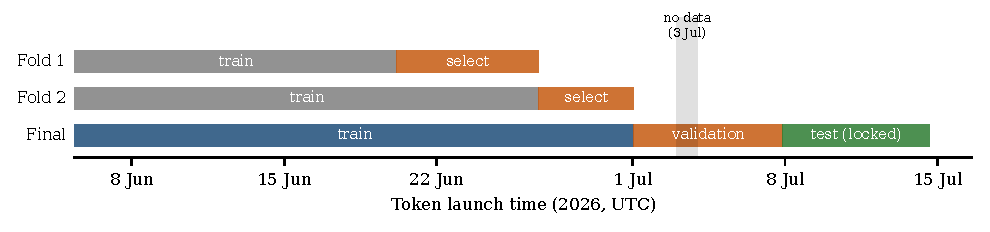
\includegraphics[width=\linewidth]{figures/fig_timeline.pdf}
\caption{Chronological splits. Walk-forward folds inside the training period were used for every model choice; the validation week was used for development reporting; the test week was scored once under a preregistered protocol. The corpus has no trades on 3 July 2026.}
\label{fig:timeline}
\end{figure}

\section{Models}
\label{sec:models}

\paragraph{Features.}
All tabular models use the same 124 features, computed strictly from information available at $T$ (Table~\ref{tab:features}, Appendix~\ref{app:features}). They fall into six groups:
\begin{itemize}
  \item \textbf{Event flow (80 features):} trade counts, buy and sell volume in SOL, buy share and flow imbalance, mean, spread and maximum trade size, price return, slope, realized volatility, drawdown and acceleration, inter-arrival times and burst intensity, each over trailing windows of 10\,s, 30\,s and 120\,s and over the token's full history;
  \item \textbf{Curve state (21):} the latest price, virtual reserves, curve progress and trade direction, plus changes, velocity and acceleration of the curve over the same windows;
  \item \textbf{Market context (14):} platform-wide launches and graduations over the last hour and day, measured up to the last completed second; trading activity in recent completed one-second buckets; and daily network statistics from the last fully completed UTC day;
  \item \textbf{Creator history (3):} information on the creating wallet's earlier launches;
  \item \textbf{Token age (2):} age in seconds and its logarithm;
  \item \textbf{Missing-data indicators (4).}
\end{itemize}

\paragraph{Simple baselines.}
We compare against six simple baselines: a \emph{volume-spike rule}, a z-score of the last 30 seconds' trade count and buy volume relative to the token's own preceding 120 seconds, in the spirit of \citet{bolz2024realtime}; a \emph{net-inflow rule}, net SOL inflow over the last 30 seconds; a \emph{curve-progress rate}, the empirical surge rate within 20 bins of curve progress, estimated on training data, following the conditioning idea of \citet{marino2026predicting}; the \emph{best single feature} by walk-forward ROC-AUC, which turned out to be drawdown over the token's full history; an L2-regularized \emph{logistic regression} with the regularization strength chosen on the folds; and a \emph{multilayer perceptron} with two hidden layers of 256 units, whose number of training epochs was set by early stopping on a holdout within the fold-2 training data. We also train an \emph{age-and-curve} model: XGBoost restricted to six features describing token age and curve position. It answers a natural question, namely whether the models learn anything beyond where a token sits on its curve and how old it is.

\paragraph{Gradient-boosted trees.}
We train XGBoost~\citep{chen2016xgboost} and LightGBM~\citep{ke2017lightgbm}. The number of boosting rounds is fixed to the median best iteration across the two walk-forward folds, and the final model is fit once on the full training period, with no early stopping on validation data. Scores are calibrated with Platt scaling~\citep{platt1999probabilistic} on a chronological holdout from the end of the training period. XGBoost with this frozen protocol is our designated \emph{champion}. A tuned LightGBM, whose configuration was chosen from 24 candidates on the folds, serves as a second tree model (Appendix~\ref{app:hparams}).

\paragraph{Multimodal Transformer.}
We also train a larger sequence model that reads raw inputs rather than engineered features. An event encoder (a six-layer Transformer with eight heads and width 256) reads up to 512 recent trades; separate two-layer encoders read the curve path, market context and creator history. Their outputs are combined by gated fusion and feed several prediction heads: surge onset at several horizons, survival, price barriers, returns and price paths. The model was pretrained with a self-supervised objective for 50,000 steps on the training population, then trained on the supervised targets for 100,000 steps, using AdamW with learning rate $3\times10^{-4}$, weight decay 0.01, 1,000 warmup steps and batch size 64. About 10 million parameters are active for the inputs used here; the full architecture, including encoders for additional data sources, has 15.7 million. A further fine-tuning stage on a multimodal subset of tokens was trained but is excluded from all results for the reasons given in Section~\ref{sec:leakage}.

\section{Evaluation Protocol}
\label{sec:protocol}

\paragraph{Metrics.}
For each model and horizon we report ROC-AUC; PR-AUC (average precision), which is more informative when positives are rare~\citep{saito2015precision}; and precision among the top 0.1\%, 0.5\%, 1\% and 2\% of observations by score.

\paragraph{Alert feed.}
To mimic a live monitor, we take, for every UTC hour, the ten highest-scoring observations, keeping at most one per token, and report the fraction of them whose token begins a surge within the next 300 seconds, compared with the base rate.

\paragraph{Event-level recall and lead time.}
Observation-level metrics can reward a model for flagging the same surge many times, so we also evaluate at the level of surge events. For each primary-definition surge whose onset falls in the evaluation window, we find the earliest observation before onset whose score is in the top 1\% (or top 2\%) of all scores. The surge is \emph{caught} if such an observation exists, and the \emph{lead time} is the gap between that observation and onset. A \emph{false alert} is a top-ranked observation whose token has no onset in the following 300 seconds; we report false alerts per caught surge.

\paragraph{Strata.}
Many observations are easy negatives: a token observed six hours after launch with no recent trades is very unlikely to surge, so pooled ROC-AUC can flatter a model. We therefore also report results within strata: by observation trigger (fixed age versus trade count); by token age; and for actively traded tokens, with at least one, or at least five, trades in the preceding 60 seconds. The trade counts used for these strata are approximated from the 30-second and 120-second feature windows.

\paragraph{Uncertainty.}
Observations from the same token are correlated, so we compute 95\% confidence intervals with a bootstrap that resamples tokens rather than observations (2,000 replicates), in the spirit of cluster-robust inference~\citep{cameron2008bootstrap}. Differences between models are computed on the same resampled tokens.

\paragraph{Protocol and preregistration.}
\begin{itemize}
  \item \emph{Development.} All choices were made on the walk-forward folds. The validation week was used to compare model families and to diagnose problems; each final configuration was scored on it once, and every such score was logged.
  \item \emph{Preregistration.} Before any test observation was read, we committed a written protocol to version control. It fixed five models (the XGBoost champion, the tuned LightGBM, the Transformer, logistic regression as the best simple baseline on validation, and the age-and-curve model), the targets, variants, strata and metrics listed above, and a commitment to report the results whatever they showed. All models were trained on the training period only and were not refit on validation data.
  \item \emph{Pipeline check.} Before the test run, we froze every model to a file with a checksum and re-ran the full scoring pipeline on the validation week; all 30 checked metrics matched the earlier reports exactly.
  \item \emph{The test run.} The scoring code refused to run unless the protocol on disk matched the committed version, and it wrote a lock file before reading any test data. The first attempt stopped during the Transformer's inference step, when a safety check refused test-period inputs, before any metric had been computed. We fixed the check and replaced the Transformer's inference loop with a streaming, single-threaded version after the multithreaded loop crashed; scoring then ran to completion. Appendix~\ref{app:prereg} documents both deviations.
\end{itemize}

\section{Results}
\label{sec:results}

\subsection{Main results on the held-out week}

Table~\ref{tab:main} reports the preregistered test results. At the 60-second horizon the base rate is 2.29\%. The XGBoost champion reaches an ROC-AUC of 0.866 and a PR-AUC of 0.112, and its top 1\% of observations has a precision of 14.6\%, 6.3 times the base rate. At the 300-second horizon the base rate is 2.73\%; the champion reaches 0.845 and 0.117, and its top 1\% has a precision of 16.2\%, 5.9 times the base rate. These figures are close to those on the validation week, where the champion scored 0.873 at 60 seconds. PR-AUC was higher on the test week (0.112 versus 0.092), largely because surges were more common that week (2.29\% versus 1.78\% of observations).

\begin{table}[t]
\centering
\caption{Preregistered test-week results. P@$k$ is the precision among the top $k$ of observations by score. The last column gives validation-week ROC-AUC and PR-AUC for reference. Bold marks the best value in a column within each horizon.}
\label{tab:main}
\tabsize
\setlength{\tabcolsep}{4pt}
\begin{tabular}{lccccccc}
\toprule
 & \multicolumn{6}{c}{Test week (preregistered, scored once)} & Validation \\
\cmidrule(lr){2-7}\cmidrule(lr){8-8}
Model & ROC-AUC & PR-AUC & P@0.1\% & P@0.5\% & P@1\% & P@2\% & ROC / PR \\
\midrule
\multicolumn{8}{l}{\emph{Onset within 60 s; base rate 2.29\%}} \\
XGBoost (champion) & 0.866 & \textbf{0.112} & 16.3\% & 15.4\% & 14.6\% & 16.0\% & 0.873 / 0.092 \\
LightGBM (tuned) & 0.866 & 0.108 & 13.0\% & 13.4\% & 13.2\% & 14.7\% & 0.873 / 0.090 \\
Logistic regression (L2) & \textbf{0.870} & 0.110 & 15.0\% & 14.3\% & 14.5\% & 14.8\% & 0.858 / 0.076 \\
Transformer & 0.852 & 0.095 & 10.5\% & 12.8\% & 12.6\% & 11.5\% & 0.858 / 0.077 \\
Age + curve XGBoost & 0.842 & 0.093 & 10.0\% & 10.6\% & 10.2\% & 9.8\% & 0.854 / 0.076 \\
\addlinespace
\multicolumn{8}{l}{\emph{Onset within 300 s; base rate 2.73\%}} \\
XGBoost (champion) & \textbf{0.845} & \textbf{0.117} & 17.1\% & 15.9\% & 16.2\% & 17.2\% & 0.858 / 0.098 \\
LightGBM (tuned) & 0.844 & 0.116 & 16.4\% & 16.1\% & 16.2\% & 16.5\% & 0.856 / 0.095 \\
Logistic regression (L2) & 0.845 & 0.114 & 15.7\% & 15.4\% & 16.1\% & 16.2\% & 0.834 / 0.078 \\
Transformer & 0.829 & 0.099 & 11.2\% & 12.9\% & 13.4\% & 12.4\% & 0.841 / 0.082 \\
Age + curve XGBoost & 0.818 & 0.097 & 11.2\% & 10.9\% & 11.0\% & 10.6\% & 0.836 / 0.080 \\
\bottomrule
\end{tabular}

\end{table}

The comparison between models is the more surprising result (Table~\ref{tab:deltas}). The champion clearly beats the Transformer, by 0.014 in ROC-AUC and 0.018 in PR-AUC at 60 seconds, with similar margins at 300 seconds, and it beats the age-and-curve model by 0.024 and 0.020. It does not clearly beat logistic regression. At 60 seconds, logistic regression has a slightly \emph{higher} ROC-AUC, by 0.0045, while the champion keeps a small PR-AUC advantage of 0.0028 whose interval nearly touches zero. At 300 seconds the two are tied on ROC-AUC, and the champion leads on PR-AUC by 0.0033. The tuned LightGBM is within 0.002 ROC-AUC of the champion at both horizons.

\begin{table}[t]
\centering
\caption{Paired differences on the test week (champion minus each model), with 95\% confidence intervals from a token-clustered bootstrap (2,000 replicates).}
\label{tab:deltas}
\tabsize
\begin{tabular}{llcc}
\toprule
Horizon & Champion minus & $\Delta$ROC-AUC [95\% CI] & $\Delta$PR-AUC [95\% CI] \\
\midrule
60 s & Logistic regression & $-$0.0045 [$-$0.0068, $-$0.0021] & +0.0028 [+0.0001, +0.0058] \\
60 s & Transformer & +0.0141 [+0.0127, +0.0155] & +0.0175 [+0.0157, +0.0196] \\
60 s & Age + curve XGBoost & +0.0236 [+0.0222, +0.0249] & +0.0196 [+0.0175, +0.0219] \\
\addlinespace
300 s & Logistic regression & +0.0001 [$-$0.0023, +0.0025] & +0.0033 [+0.0008, +0.0060] \\
300 s & Transformer & +0.0153 [+0.0138, +0.0167] & +0.0180 [+0.0162, +0.0200] \\
300 s & Age + curve XGBoost & +0.0262 [+0.0248, +0.0276] & +0.0203 [+0.0183, +0.0224] \\
\bottomrule
\end{tabular}

\end{table}

The rule-based baselines were not part of the test protocol. On the validation week they were far weaker (Table~\ref{tab:baselines}, Appendix~\ref{app:extra}): the volume-spike and net-inflow rules reached ROC-AUC 0.61 and 0.54 at 60 seconds, the curve-progress rate 0.65, and the best single feature 0.68. The multilayer perceptron reached 0.843, below logistic regression (0.858).

\subsection{Easy and hard observations}

Pooled ROC-AUC is driven partly by observations that are easy to rule out. Table~\ref{tab:strata} breaks test performance down by stratum. At 60 seconds, the champion's ROC-AUC is 0.921 among fixed-age observations but 0.710 among trade-count observations, which are taken during bursts of activity. By token age, it rises from 0.676 for tokens younger than 30 seconds to 0.768 for 30 seconds to 2 minutes, 0.828 for 2 to 10 minutes and 0.866 for 10 minutes to an hour; observations older than an hour contain no positives. Among tokens with at least one trade in the preceding minute, ROC-AUC is 0.768 at 60 seconds and 0.731 at 300 seconds (Appendix Table~\ref{tab:strata300}).

We regard the active-token numbers as the most honest summary of how well surge onset can be anticipated: well above chance, but far from the pooled figures. Within strata, no model family wins everywhere. On the test week, logistic regression has the highest ROC-AUC among the youngest tokens (0.687), among trade-count observations (0.743) and among active tokens (0.790 and 0.802), whereas XGBoost is best for tokens between 30 seconds and 10 minutes old. On the validation week the ordering among active tokens was the reverse (XGBoost 0.787, Transformer 0.775, logistic regression 0.769; Table~\ref{tab:valstrata}). We therefore do not claim that any one of these families is better at the hard cases.

\begin{table}[t]
\centering
\caption{Test-week ROC-AUC by stratum, 60-second horizon. Bold marks the best model in each row. Observations older than one hour contain no positives and are omitted. Activity strata are approximated from the 30\,s and 120\,s feature windows.}
\label{tab:strata}
\tabsize
\setlength{\tabcolsep}{4pt}
\begin{tabular}{lrrccccc}
\toprule
 & & & \multicolumn{5}{c}{ROC-AUC} \\
\cmidrule(lr){4-8}
Stratum & $n$ & Prevalence & XGB & LGBM & Logistic & Transf. & Age+curve \\
\midrule
Fixed-age observations & 914{,}583 & 1.74\% & 0.921 & \textbf{0.921} & 0.915 & 0.907 & 0.909 \\
Trade-count observations & 358{,}858 & 3.70\% & 0.710 & 0.711 & \textbf{0.743} & 0.702 & 0.666 \\
Age $<$ 30 s & 434{,}610 & 6.19\% & 0.676 & 0.674 & \textbf{0.687} & 0.657 & 0.647 \\
Age 30 s -- 2 min & 256{,}034 & 0.73\% & \textbf{0.768} & 0.759 & 0.695 & 0.702 & 0.641 \\
Age 2 -- 10 min & 215{,}367 & 0.17\% & \textbf{0.828} & 0.806 & 0.706 & 0.792 & 0.694 \\
Age 10 min -- 1 h & 188{,}125 & 0.02\% & 0.866 & 0.890 & 0.771 & \textbf{0.937} & 0.790 \\
Active: $\geq$1 trade in last 60 s & 644{,}678 & 2.58\% & 0.768 & 0.770 & \textbf{0.790} & 0.754 & 0.718 \\
Active: $\geq$5 trades in last 60 s & 250{,}692 & 1.88\% & 0.772 & 0.773 & \textbf{0.802} & 0.746 & 0.683 \\
\bottomrule
\end{tabular}

\end{table}

\subsection{How much warning, and how many surges}

The test week contains 12,225 primary-definition surges. With the 60-second model, the top-1\% threshold catches 8.4\% of them, with a median lead time of 5.2 seconds (interquartile range 2.1 to 17.7 seconds) and 10.4 false alerts per caught surge; the top-2\% threshold catches 23.1\%, with a median lead of 4.8 seconds and 7.5 false alerts per caught surge (Table~\ref{tab:recall}). The 300-second model catches 10.3\% and 23.9\% at the same thresholds, also with median leads of about five seconds. The alert feed tells a similar story: of the ten highest-scoring tokens in each hour of the test week, an average of 15.2\% began a surge within 300 seconds, against a base rate of 2.73\%, a lift of 5.6.

\begin{table}[t]
\centering
\caption{Event-level recall on the test week (12,225 primary surges). Lead time is measured from the earliest alerted observation to onset. False alerts are top-ranked observations whose token has no onset in the following 300 seconds.}
\label{tab:recall}
\tabsize
\setlength{\tabcolsep}{4pt}
\begin{tabular}{llrrrrrrrr}
\toprule
 & & & & \multicolumn{5}{c}{Lead time (s), percentiles} & False alerts \\
\cmidrule(lr){5-9}
Scores & Threshold & Caught & $n$ caught & p10 & p25 & p50 & p75 & p90 & per catch \\
\midrule
60 s & Top 1\% & 8.4\% & 1{,}033 & 0.6 & 2.1 & 5.2 & 17.7 & 64.5 & 10.4 \\
60 s & Top 2\% & 23.1\% & 2{,}818 & 1.2 & 2.4 & 4.8 & 14.4 & 62.3 & 7.5 \\
300 s & Top 1\% & 10.3\% & 1{,}262 & 0.9 & 2.2 & 5.0 & 17.7 & 68.2 & 8.5 \\
300 s & Top 2\% & 23.9\% & 2{,}918 & 1.2 & 2.5 & 5.0 & 15.2 & 64.9 & 7.2 \\
\bottomrule
\end{tabular}

\end{table}

The warning is short, and a model that merely reacts to a surge already under way could look good on pooled metrics without being useful. The stricter variants address this (Table~\ref{tab:variants}). Removing observations whose surge has already started leaves the champion's 60-second ROC-AUC essentially unchanged (0.865) and raises its top-1\% precision to 19.9\%. Requiring at least five seconds of warning lowers ROC-AUC to 0.848 at 60 seconds and 0.823 at 300 seconds. The signal therefore does not depend on detecting surges that have already begun.

\begin{table}[t]
\centering
\caption{Champion results on the test week under the stricter evaluation variants.}
\label{tab:variants}
\tabsize
\begin{tabular}{llrrccc}
\toprule
Horizon & Evaluation set & Positives & Prevalence & ROC-AUC & PR-AUC & P@1\% \\
\midrule
60 s & All observations & 29{,}212 & 2.29\% & 0.866 & 0.112 & 14.6\% \\
60 s & (a) Already-started removed & 29{,}212 & 2.66\% & 0.865 & 0.134 & 19.9\% \\
60 s & (c) $\geq$5 s warning required & 17{,}391 & 1.60\% & 0.848 & 0.069 & 10.4\% \\
300 s & All observations & 34{,}783 & 2.73\% & 0.845 & 0.117 & 16.2\% \\
300 s & (a) Already-started removed & 34{,}783 & 3.17\% & 0.845 & 0.138 & 20.9\% \\
300 s & (c) $\geq$5 s warning required & 22{,}962 & 2.12\% & 0.823 & 0.078 & 11.9\% \\
\bottomrule
\end{tabular}

\end{table}

\subsection{Surge definitions and large surges}

On the validation week, results were similar across the three surge definitions, with 60-second ROC-AUC of 0.878 (conservative), 0.873 (primary) and 0.877 (aggressive); PR-AUC moved with prevalence, as expected (Table~\ref{tab:labels}). Large surges are harder. For the 2$\times$ target on the test week (prevalence 0.91\%), the champion reaches an ROC-AUC of 0.838 and a PR-AUC of 0.033, and its hourly alert feed has a lift of 3.6. On the validation week it caught only 3.7\% of 2$\times$ surges at the top-1\% threshold and 7.7\% at the top-2\% threshold. Whether a surge will be large appears to be much less predictable from pre-onset information than whether a surge will happen.

\begin{table}[t]
\centering
\caption{Sensitivity to the surge definition (validation week) and results for the 2$\times$ target.}
\label{tab:labels}
\tabsize
\begin{tabular}{llrrcc}
\toprule
Split & Target & Positives & Prevalence & ROC-AUC & PR-AUC \\
\midrule
Validation & Conservative, 60 s & 12{,}291 & 0.96\% & 0.878 & 0.054 \\
Validation & Primary, 60 s & 22{,}221 & 1.78\% & 0.873 & 0.092 \\
Validation & Aggressive, 60 s & 35{,}953 & 2.82\% & 0.877 & 0.138 \\
Validation & 2$\times$ surge within 300 s & 6{,}867 & 0.56\% & 0.853 & 0.023 \\
Test & 2$\times$ surge within 300 s & 11{,}419 & 0.91\% & 0.838 & 0.033 \\
\bottomrule
\end{tabular}

\end{table}

\subsection{Why the model family matters so little}

Three observations suggest that the signal lies mainly in a small number of well-chosen state variables. Logistic regression nearly matches gradient-boosted trees overall and beats them among active tokens on the test week; tuning the trees on the walk-forward folds changed validation ROC-AUC by less than 0.005; and a Transformer that reads up to 512 raw trades does worse overall than a linear model on summary features. Our Transformer was trained with one configuration and modest tuning, so a stronger sequence model may exist. Still, the direction of the result matches findings on tabular benchmarks~\citep{grinsztajn2022tree,shwartzziv2022tabular,mcelfresh2023neural}, and it suggests that, at this horizon, the order and fine timing of individual trades add little beyond what windowed aggregates already capture.

\subsection{What the models use}

We computed TreeSHAP attributions~\citep{lundberg2020trees} for the 300-second champion on a fixed sample of 50,000 validation observations (Figure~\ref{fig:shap}). Summed over groups, mean absolute attribution is highest for token age (0.96), followed by curve state (0.74), event flow (0.47), market context (0.13) and creator history (0.05). The single most important features are token age, virtual token reserves and price. Removing the two age features lowers validation ROC-AUC at 300 seconds from 0.858 to 0.841, while removing any other single group costs less than 0.007, which indicates that the groups overlap heavily. The age-and-curve model alone reaches 0.842 on the test week at 60 seconds, and the rest of the feature set adds a modest but reliable 0.024. Put simply, the models learn that surges happen mostly to young tokens early on their curves, and then use recent trading activity to rank tokens within that group.

\begin{figure}[t]
\centering
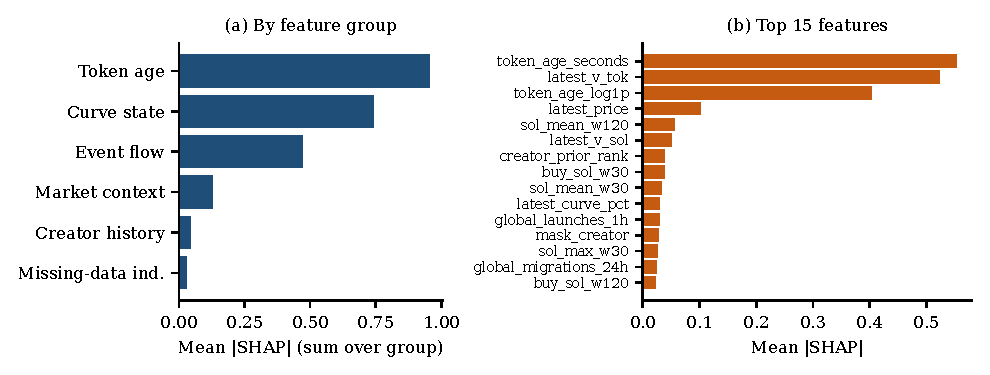
\includegraphics[width=\linewidth]{figures/fig_shap.pdf}
\caption{TreeSHAP attributions for the 300-second champion on 50,000 validation observations: (a) mean absolute attribution summed within each feature group; (b) the 15 most important individual features.}
\label{fig:shap}
\end{figure}

\subsection{Stability over time and the value of more data}

Across the days of the validation week, the champion's 300-second ROC-AUC ranged from 0.841 to 0.895 (Figure~\ref{fig:stability}a). When we trained the tuned configurations on the most recent 25\%, 50\%, 75\% and 100\% of the training period, validation PR-AUC at 60 seconds was highest with all the data for both LightGBM (0.077 at 25\% to 0.090 at 100\%) and XGBoost (0.080 to 0.091), and the curves had not leveled off (Figure~\ref{fig:stability}b). A longer history is the most promising way to improve these results.

\begin{figure}[t]
\centering
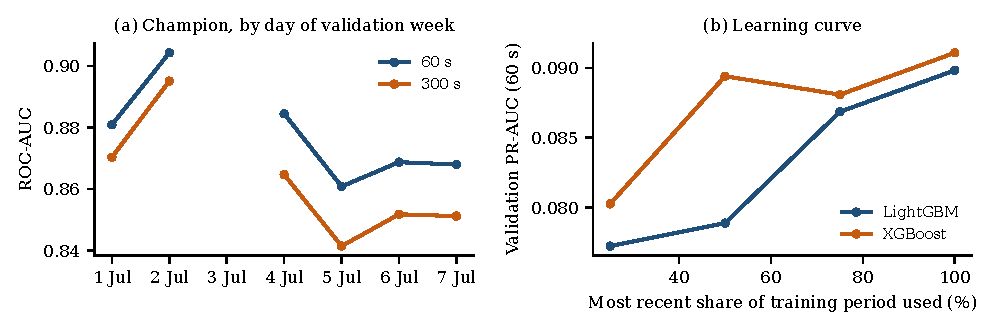
\includegraphics[width=\linewidth]{figures/fig_stability.pdf}
\caption{(a) Champion ROC-AUC on each day of the validation week; there are no data for 3 July. (b) Validation PR-AUC at 60 seconds when training on the most recent share of the training period.}
\label{fig:stability}
\end{figure}

\subsection{Predictable is not profitable}

A model that anticipates surges might seem to promise easy profits. Our data say otherwise (Table~\ref{tab:econ}). On the validation week, the median simple return over the five minutes after an observation was $-9.1\%$ across all eligible observations with a recorded return, and $-40.2\%$ (mean $-10.8\%$) for the champion's top 1\%. The same top-ranked observations had a median maximum favorable excursion of $+31.5\%$ and a median maximum adverse excursion of $-41.2\%$ over those five minutes: prices often rose first and then fell sharply. These are gross returns measured from the last trade price at $T$. They ignore fees and slippage and assume entry at exactly $T$; our data do not include prices for entries delayed by a realistic few seconds, and real outcomes would almost certainly be worse. The observations a model can most easily flag sit in the middle of bursts of activity that frequently reverse, which is what one would expect in a market where any obvious edge is competed away by faster participants.

\begin{table}[t]
\centering
\caption{Five-minute outcomes on the validation week (descriptive; gross of fees and slippage). MFE and MAE are the maximum favorable and adverse price excursions within five minutes.}
\label{tab:econ}
\tabsize
\begin{tabular}{lrcccc}
\toprule
 & & \multicolumn{2}{c}{5-min return} & Median & Median \\
\cmidrule(lr){3-4}
Observations & $n$ & Median & Mean & MFE & MAE \\
\midrule
All eligible observations & 516{,}383 & $-$9.1\% & $-$8.9\% & 1.1\% & $-$15.7\% \\
Champion top 1\% & 9{,}843 & $-$40.2\% & $-$10.8\% & 31.5\% & $-$41.2\% \\
\bottomrule
\end{tabular}

\end{table}

\section{Case Study: Selection Leakage in On-Chain Data Acquisition}
\label{sec:leakage}

Early in this project, a richer version of the dataset seemed to deliver a large improvement. The improvement was not real. We describe how it arose because the same mistake is easy to make in any study that samples on-chain data to save cost.

\paragraph{The setting.}
For a stratified random sample of 4,000 tokens (3,623 of them in the training and validation periods), we gathered four extra data sources: transaction-level metadata from a Solana RPC node (fees, compute units and success flags), token-balance changes describing ownership, a wallet--token trading graph, and the earlier trading histories of the wallets involved. Fetching every transaction for every token was too expensive, so the acquisition code fetched a small number of transactions per token (at most 16), chosen to cover the token's history: the first and last trades, the median buy and sell, the smallest and largest trades, the trades at the lowest and highest curve progress, and an evenly spaced grid over the token's lifetime.

\paragraph{The leak.}
Every fetched transaction carried an accurate timestamp, and every feature used only transactions dated before $T$, so per-record timestamp checks passed. The problem was \emph{which} transactions existed in the data at all. The selection was made over each token's entire lifetime, including trades after $T$. As a result, the number of fetched transactions dated before $T$ encoded information about the future: if the token's largest trade or curve peak was still to come, fewer of the fetched transactions fell before $T$ (Figure~\ref{fig:leak}). That count, a feature named \texttt{micro\_n}, was the strongest feature in the richer tree model, with roughly three times the importance of the next one.

\begin{figure}[t]
\centering
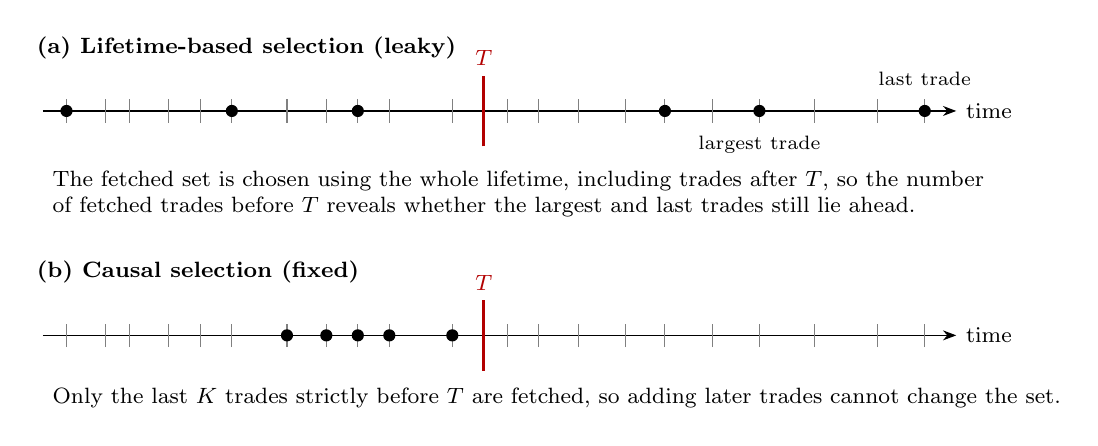
\begin{tikzpicture}[x=1cm,y=1cm,>=Stealth,font=\footnotesize]
  % (a) lifetime-based selection
  \node[anchor=west] at (-0.2,3.4) {\textbf{(a) Lifetime-based selection (leaky)}};
  \draw[->] (0,2.6) -- (11.6,2.6) node[right] {time};
  \foreach \x in {0.3,0.8,1.1,1.6,2.0,2.4,3.1,3.6,4.0,4.4,5.2,5.9,6.3,6.8,7.4,7.9,8.5,9.1,9.8,10.6,11.2}
    \draw[gray] (\x,2.45) -- (\x,2.75);
  \foreach \x in {0.3,2.4,4.0,7.9,9.1,11.2}
    \fill[black] (\x,2.6) circle (2.2pt);
  \draw[very thick,red!70!black] (5.6,2.15) -- (5.6,3.05);
  \node[red!70!black,above] at (5.6,3.05) {$T$};
  \node[anchor=north,align=center,font=\scriptsize] at (9.1,2.4) {largest trade};
  \node[anchor=south,align=center,font=\scriptsize] at (11.2,2.8) {last trade};
  \node[anchor=west,align=left] at (0,1.55) {The fetched set is chosen using the whole lifetime, including trades after $T$, so the number\\of fetched trades before $T$ reveals whether the largest and last trades still lie ahead.};
  % (b) causal selection
  \node[anchor=west] at (-0.2,0.55) {\textbf{(b) Causal selection (fixed)}};
  \draw[->] (0,-0.25) -- (11.6,-0.25) node[right] {time};
  \foreach \x in {0.3,0.8,1.1,1.6,2.0,2.4,3.1,3.6,4.0,4.4,5.2,5.9,6.3,6.8,7.4,7.9,8.5,9.1,9.8,10.6,11.2}
    \draw[gray] (\x,-0.4) -- (\x,-0.1);
  \foreach \x in {3.1,3.6,4.0,4.4,5.2}
    \fill[black] (\x,-0.25) circle (2.2pt);
  \draw[very thick,red!70!black] (5.6,-0.7) -- (5.6,0.2);
  \node[red!70!black,above] at (5.6,0.2) {$T$};
  \node[anchor=west,align=left] at (0,-1.05) {Only the last $K$ trades strictly before $T$ are fetched, so adding later trades cannot change the set.};
\end{tikzpicture}
\caption{How the transaction-selection rule leaked future information. Grey ticks are trades; black dots are the trades whose transactions were fetched.}
\label{fig:leak}
\end{figure}

\paragraph{The evidence.}
On the subset's validation tokens (Table~\ref{tab:leak}), \texttt{micro\_n} was identical to the number of selected transactions before $T$ for 100\% of observations. On its own, \texttt{micro\_n} had an ROC-AUC of 0.125 for 60-second onset, that is, 0.875 once its sign is flipped. A single yes/no indicator, ``the token's largest trade happens after $T$'', reached 0.825 on its own, almost as high as the entire set of legitimate broad features (0.835). A tree model using all broad and rich features reached 0.917. Adding the explicit share of selected transactions dated before $T$, a deliberate ``canary'' feature, raised it further to 0.921, while removing the microstructure features dropped it to 0.881. Keeping only the two rich sources whose selection was causal, the trading graph and the wallet histories, gave 0.841, statistically indistinguishable from broad features alone. The ownership data reused the same transaction selection and inherited the leak. The fine-tuned multimodal Transformer depended on it as well: hiding the microstructure inputs at inference time lowered its ROC-AUC from 0.850 to 0.745.

\begin{table}[t]
\centering
\caption{Leak case study on the multimodal subset (validation tokens; 8,027 eligible observations of 600 tokens; 60-second horizon). Single-feature ROC-AUC values below 0.5 mean that lower values of the feature predict onset.}
\label{tab:leak}
\tabsize
\begin{tabular}{lcc}
\toprule
Model or feature (multimodal subset, validation tokens) & ROC-AUC & PR-AUC \\
\midrule
Broad features only (arm A) & 0.835 & 0.074 \\
Broad + all rich features (arm B) & 0.917 & 0.114 \\
Arm B + leak canary (share of fetched txs before $T$) & 0.921 & 0.120 \\
Arm B without microstructure & 0.881 & 0.108 \\
Broad + causally selected rich sources only & 0.841 & 0.070 \\
\midrule
\texttt{micro\_n} alone & 0.125 & -- \\
``Largest trade is after $T$'' alone & 0.825 & -- \\
Causal trade count before $T$ alone & 0.305 & -- \\
\bottomrule
\end{tabular}

\end{table}

\paragraph{A second failure: the metric.}
While investigating, we also found a bug in the project's own ROC-AUC function. A ranking step indexed labels and ranks in different orders, and on predictions whose true ROC-AUC was 0.894 the function reported 0.535. Had we trusted it, we would have discarded a working model. We found the bug only because we recomputed every reported metric with an independent implementation.

\paragraph{What we changed.}
We quarantined the leaky data sources and every result derived from them, including the fine-tuned Transformer stage. We replaced lifetime-based selection with a causal rule that fetches the last $K$ trades strictly before $T$, and added a regression test that appending arbitrary trades after $T$ does not change the selected set; the old function fails it and the new one passes. We also fixed the metric and tested it against a reference implementation on data with ties.

\paragraph{Lessons.}
Five practices would have caught these problems earlier: audit how records were \emph{selected}, not only their timestamps; test that features are invariant to appending future events; add canary features that encode the suspected leak and see whether performance jumps; compute every reported metric with two independent implementations; and treat any large, surprising gain as a leak until shown otherwise. None of these is new on its own~\citep{kapoor2023leakage,lopezdeprado2018advances}, but selection leakage of this kind is easy to miss and likely to recur in on-chain research, where cost-constrained sampling from RPC nodes is common.

\section{Discussion}
\label{sec:discussion}

\paragraph{What the predictability means.}
Surge onset on pump.fun is not random. It concentrates among young tokens early on their bonding curves, and recent trading activity sharpens the ranking further. Part of this is mechanical: a token that is a few seconds old and already attracting buyers is simply in the phase of life when surges happen. The active-token results show that the models also distinguish among tokens that are all in that phase, though with ROC-AUC values in the mid-0.7s rather than the high 0.8s.

\paragraph{Who could use this.}
The most defensible uses are protective. A wallet or platform could flag tokens entering a surge phase and show users the poor median outcomes that follow, and researchers and regulators can use surge onsets, and the benchmark itself, to study manipulation and market quality. Our results argue against using such a model as a trading signal by itself.

\paragraph{Limitations.}
\begin{itemize}
  \item \emph{Short window.} The data cover 39 days of a single platform, and the market changes quickly; the corpus documentation reports, for example, a steep rise in the graduation rate over the window and a shift in one curve-progress field after 4 July~\citep{slinkdev2026corpus}. Results may not hold in other periods or on other launchpads.
  \item \emph{Data gaps.} One day (3 July) has no recorded trades, and some tokens' trades carry no prices; affected labels are excluded rather than imputed.
  \item \emph{Detector-defined surges.} Surges are defined by a detector we designed. We report alternative definitions, but other reasonable definitions could give different numbers.
  \item \emph{Gross returns.} Our return figures ignore fees, slippage and execution delay.
  \item \emph{Approximate strata.} The active-token strata are approximated from feature windows rather than exact trade counts.
  \item \emph{One deep model.} The Transformer represents one reasonable design with limited tuning, not the best possible sequence model.
  \item \emph{Multimodal data excluded.} After discovering the leak, we excluded the multimodal subset from the main results, so we cannot say whether causally collected transaction-level data would help.
  \item \emph{Test-run deviations.} The test run deviated from the planned procedure in two documented ways that did not affect any model or metric (Appendix~\ref{app:prereg}).
  \item \emph{Manipulation not distinguished.} We make no claim about whether individual surges were organic or coordinated.
\end{itemize}

\paragraph{Ethics and dual use.}
A surge-onset model could, in principle, help automated traders act ahead of other participants. We think the added risk is limited: the warning is a few seconds, the highest-ranked observations are followed by large median losses, and faster participants already act on similar information. We use only public on-chain data, we do not identify or profile individual wallets, and we do not release a trading strategy.

\section{Conclusion}
\label{sec:conclusion}

We asked whether the start of a memecoin price surge can be predicted seconds ahead using only on-chain information. On a locked, preregistered final week of pump.fun data, it can, to a useful but limited degree. The best models rank surge onsets about six times above the base rate among their top alerts, with around five seconds of warning. A simple logistic regression does about as well as gradient-boosted trees, and better than a much larger Transformer. High predictability coexists with steep losses for anyone who buys on the signal. We also showed how a plausible data-acquisition shortcut can manufacture an impressive but false result. Extending the data to longer periods and other launchpads, and collecting richer transaction-level data under strictly causal rules, are the natural next steps.

\section*{Data and Code Availability}
The source data are the public PumpFun Launch-to-Graduation Corpus~\citep{slinkdev2026corpus}. The code for data processing, labeling, model training and evaluation, together with the evaluation reports, the preregistered test protocols and the scripts that generate every table and figure in this paper, is available at \url{https://github.com/heyronith/trencher}.

\section*{Acknowledgments}
We thank the maintainers of the PumpFun Launch-to-Graduation Corpus for making their data public. This research received no external funding. AI assistants were used for research planning, code generation and review, and drafting and editing of the text. The author designed and directed the study, ran all experiments, checked the reported results, and takes full responsibility for the content of this paper.


\bibliographystyle{plainnat}
\bibliography{references}

\clearpage
\appendix
\section{Feature List}
\label{app:features}

\begin{table}[h]
\centering
\caption{The 124 features used by all tabular models. Windowed features are computed over trailing windows of 10\,s, 30\,s and 120\,s and over the token's full history, and each name below stands for all of its windows.}
\label{tab:features}
\tabsize
\begin{tabularx}{\linewidth}{lrX}
\toprule
Group & $n$ & Features (windowed features appear once per window: 10 s, 30 s, 120 s and full history) \\
\midrule
Event flow & 80 & \texttt{event\_count}, \texttt{buy\_count}, \texttt{sell\_count}, \texttt{buy\_fraction}, \texttt{buy\_sol}, \texttt{sell\_sol}, \texttt{net\_sol}, \texttt{flow\_imbalance}, \texttt{sol\_mean}, \texttt{sol\_std}, \texttt{sol\_max}, \texttt{price\_return}, \texttt{price\_slope}, \texttt{realized\_vol}, \texttt{drawdown}, \texttt{price\_accel}, \texttt{interarrival\_mean}, \texttt{interarrival\_std}, \texttt{burst\_intensity}, \texttt{intensity\_accel} \\
Curve state & 21 & \texttt{reserve\_delta\_sol}, \texttt{curve\_delta}, \texttt{curve\_velocity}, \texttt{curve\_accel}, \texttt{latest\_price}, \texttt{latest\_v\_sol}, \texttt{latest\_v\_tok}, \texttt{latest\_curve\_pct}, \texttt{latest\_is\_buy} \\
Market context & 14 & \texttt{global\_launches\_1h}, \texttt{global\_launches\_24h}, \texttt{global\_migrations\_1h}, \texttt{global\_migrations\_24h}, \texttt{daily\_network\_launches}, \texttt{daily\_network\_graduations}, \texttt{daily\_network\_trades}, \texttt{daily\_network\_buy\_volume\_sol}, \texttt{daily\_network\_graduation\_rate}, \texttt{global\_bucket\_trades\_sum}, \texttt{global\_bucket\_buy\_sol\_sum}, \texttt{global\_bucket\_sell\_sol\_sum}, \texttt{global\_bucket\_imbalance}, \texttt{global\_bucket\_unique\_mints\_mean} \\
Creator history & 3 & \texttt{creator\_prior\_rank}, \texttt{creator\_prior\_is\_mayhem}, \texttt{creator\_history\_n} \\
Token age & 2 & \texttt{token\_age\_seconds}, \texttt{token\_age\_log1p} \\
Missing-data indicators & 4 & \texttt{mask\_events}, \texttt{mask\_curve}, \texttt{mask\_creator}, \texttt{mask\_global} \\
\bottomrule
\end{tabularx}

\end{table}

\section{Surge Detector Parameters}
\label{app:detector}

\begin{table}[h]
\centering
\caption{Parameters of the three surge definitions. The primary definition is used throughout unless stated otherwise. Parameters were fixed before any model was trained.}
\label{tab:detector}
\tabsize
\begin{tabular}{lccc}
\toprule
Parameter & Conservative & Primary & Aggressive \\
\midrule
Window (s) & 45 & 30 & 20 \\
Baseline (s) & 180 & 120 & 90 \\
Confirmation window (s) & 90 & 60 & 45 \\
Minimum price rise in window & 25\% & 15\% & 8\% \\
Trade-rate multiple vs.\ baseline & 4$\times$ & 3$\times$ & 2$\times$ \\
Minimum distinct buyers & 5 & 3 & 2 \\
Buy-volume multiple vs.\ baseline & 3$\times$ & 2.5$\times$ & 2$\times$ \\
Minimum trades in window & 8 & 5 & 3 \\
Minimum subsequent rise & 50\% & 25\% & 15\% \\
Peak search after onset (s) & 1800 & 1800 & 1800 \\
Exhaustion drawdown from peak & 25\% & 20\% & 15\% \\
\bottomrule
\end{tabular}

\end{table}

The exhaustion drawdown marks the end of a surge (the first point after the peak at which the price has fallen by that fraction). It is recorded for description only and does not affect the labels.

\section{Hyperparameters}
\label{app:hparams}

\begin{itemize}
  \item \textbf{XGBoost (champion and age-and-curve model):} learning rate 0.05, maximum depth 8, row and column subsampling 0.8, histogram tree method, positive-class weight equal to the ratio of negatives to positives in the training data; 50 boosting rounds for both horizons (64 for the 2$\times$ target), fixed to the median best iteration on the walk-forward folds.
  \item \textbf{LightGBM (tuned):} learning rate 0.05, 63 leaves, at least 100 observations per leaf, bagging fraction 0.8 every iteration, feature fraction 0.8, no class weighting; 50 boosting rounds. Chosen from a grid of 24 configurations by mean PR-AUC on the two walk-forward folds.
  \item \textbf{Logistic regression:} standardized features, L2 penalty, regularization strength $C$ chosen from the set $\{0.01, 0.1, 1, 10\}$ by the mean PR-AUC on the walk-forward folds ($C=0.01$ for both horizons).
  \item \textbf{Multilayer perceptron:} two hidden layers of 256 ReLU units, Adam with learning rate $10^{-3}$, L2 penalty $10^{-4}$, batch size 2,048; number of epochs set by early stopping on a holdout within the fold-2 training data, then refit on the full training period.
  \item \textbf{Transformer:} see Section~\ref{sec:models}.
\end{itemize}

\section{Additional Results}
\label{app:extra}

\begin{table}[h]
\centering
\caption{All baselines on the validation week. Alert lift is the hourly top-ten precision divided by the base rate. Confidence intervals for the champion's PR-AUC advantage were computed for the 300-second horizon.}
\label{tab:baselines}
\tabsize
\setlength{\tabcolsep}{4pt}
\begin{tabular}{lccccc}
\toprule
Model & ROC-AUC & PR-AUC & P@1\% & Alert lift & Champion $-$ model, $\Delta$PR [95\% CI] \\
\midrule
\multicolumn{6}{l}{\emph{Onset within 60 s}} \\
Volume-spike z-score (rule) & 0.615 & 0.023 & 0.8\% & 0.3 & -- \\
Net SOL inflow, 30 s (rule) & 0.544 & 0.021 & 0.6\% & 0.1 & -- \\
Curve-progress rate & 0.651 & 0.036 & 6.2\% & 3.4 & -- \\
Best single feature & 0.683 & 0.030 & 2.6\% & 1.7 & -- \\
MLP (2$\times$256) & 0.843 & 0.068 & 8.9\% & 4.9 & -- \\
Logistic regression (L2) & 0.858 & 0.076 & 12.0\% & 4.8 & -- \\
XGBoost (champion) & 0.873 & 0.092 & 12.6\% & 5.7 & -- \\
\addlinespace
\multicolumn{6}{l}{\emph{Onset within 300 s}} \\
Volume-spike z-score (rule) & 0.617 & 0.028 & 1.5\% & 0.3 & +0.071 [+0.068, +0.074] \\
Net SOL inflow, 30 s (rule) & 0.543 & 0.025 & 1.0\% & 0.1 & +0.073 [+0.070, +0.077] \\
Curve-progress rate & 0.634 & 0.039 & 6.3\% & 3.4 & +0.059 [+0.056, +0.063] \\
Best single feature & 0.664 & 0.033 & 2.9\% & 1.7 & +0.065 [+0.062, +0.069] \\
MLP (2$\times$256) & 0.809 & 0.071 & 10.6\% & 5.3 & +0.027 [+0.024, +0.031] \\
Logistic regression (L2) & 0.834 & 0.078 & 12.4\% & 4.5 & +0.020 [+0.017, +0.023] \\
XGBoost (champion) & 0.858 & 0.098 & 14.2\% & 6.2 & -- \\
\bottomrule
\end{tabular}

\end{table}

\begin{table}[h]
\centering
\caption{Test-week ROC-AUC by stratum, 300-second horizon.}
\label{tab:strata300}
\tabsize
\setlength{\tabcolsep}{4pt}
\begin{tabular}{lrrccccc}
\toprule
 & & & \multicolumn{5}{c}{ROC-AUC} \\
\cmidrule(lr){4-8}
Stratum & $n$ & Prevalence & XGB & LGBM & Logistic & Transf. & Age+curve \\
\midrule
Fixed-age observations & 913{,}875 & 2.06\% & \textbf{0.902} & 0.902 & 0.895 & 0.887 & 0.886 \\
Trade-count observations & 358{,}564 & 4.45\% & 0.684 & 0.684 & \textbf{0.706} & 0.672 & 0.640 \\
Age $<$ 30 s & 434{,}227 & 6.95\% & 0.664 & 0.662 & \textbf{0.670} & 0.642 & 0.634 \\
Age 30 s -- 2 min & 255{,}839 & 1.32\% & \textbf{0.720} & 0.695 & 0.644 & 0.665 & 0.608 \\
Age 2 -- 10 min & 215{,}166 & 0.50\% & \textbf{0.814} & 0.779 & 0.707 & 0.775 & 0.661 \\
Age 10 min -- 1 h & 187{,}981 & 0.07\% & 0.901 & 0.914 & 0.828 & \textbf{0.915} & 0.848 \\
Active: $\geq$1 trade in last 60 s & 644{,}125 & 3.26\% & 0.731 & 0.729 & \textbf{0.740} & 0.715 & 0.681 \\
Active: $\geq$5 trades in last 60 s & 250{,}473 & 2.59\% & 0.719 & 0.714 & \textbf{0.734} & 0.698 & 0.645 \\
\bottomrule
\end{tabular}

\end{table}

\begin{table}[h]
\centering
\caption{Validation-week ROC-AUC among active tokens (60-second horizon), for comparison with Table~\ref{tab:strata}.}
\label{tab:valstrata}
\tabsize
\begin{tabular}{lccc}
\toprule
Validation week, 60 s & XGBoost & Logistic & Transformer \\
\midrule
Active: $\geq$1 trade in last 60 s & 0.787 & 0.769 & 0.775 \\
Active: $\geq$5 trades in last 60 s & 0.785 & 0.767 & 0.761 \\
\bottomrule
\end{tabular}

\end{table}

\section{Preregistration and Deviations}
\label{app:prereg}

The test protocol was committed to the project repository before any test observation was read, and an amendment adding the activity and age strata, the 2$\times$ target and the age-and-curve model was committed before the scoring code was written (commit \texttt{3299ee8}). The scoring code refused to run unless the protocol file matched the committed version, the working tree was clean and no earlier test results existed, and it wrote a lock file before reading any test data. The final report is in commit \texttt{704bd70}.

Two deviations occurred, both in the Transformer's inference step and both before any metric was computed. First, a safety check in the data loader still refused test-period inputs, which stopped the first run; the check was changed to accept test inputs only while the lock file is present. Second, the standard multithreaded CPU inference loop then crashed during the long run; it was replaced with a streaming, single-threaded loop that computes only the surge-onset outputs. No model, feature, target or metric was changed, and the lock file from the first attempt was kept as a record.


\end{document}
